\documentclass[a4paper]{article}

\usepackage[english]{babel}
\usepackage[utf8]{inputenc}
\usepackage{float}
\usepackage{amsmath}
\usepackage{graphicx}
\usepackage{subfigure}
\usepackage{multirow}
\usepackage{natbib}
\usepackage[colorinlistoftodos]{todonotes}

\title{\bfseries{COMP90016 -- Assignment 2 }}
\author{Haonan Li}

\date{\today}

\begin{document}
\maketitle

\section{Introduction}
\label{sec:introduction}

This assignment consists of three tasks. 

In the first task, we discuss the application of HMMs to CNV detection in theory. The second task is an implementation of a CNV detection algorithm using circular binary segmentation. In the final task, we discuss the biology of a particular cancer sample.

\section{Task1}

The lectures introduced a HMM designed to detect CNVs in a haploid organism. It consisted of three states: One for the normal copy number (CP1) and two alternate copy number states (Cp0, CP2).\\

\noindent\textbf{Question 1} How would you adapt this approach to a diploid organism, such as human (with states representing different integer copy numbers)? \\

\noindent\textbf{Answer}: For a diploid organism. The normal copy number of chromosome is 2. Take account of copy number changes. four alternate copy number states should be used (CP0, CP1, CP3, CP4). All of them maybe exist in the real world. However, it should be adjust according to the datasets. If there are some bins with 5 copy numbers. We might add CP5 to the state set. More details from document of CNV\footnote{http://www.completegenomics.com/documents/CNV+Methods.pdf}. In principle, model parameters can all be estimated by expectation-maximization (EM) by the Baum-Welch algorithm. Some assumptions: a) Coverage depends on the number of copies of a given reference segment in the genome of interest. b) Copy number is assumed to be integer-valued. c) Coverage is assumed to be linearly related to copy number. d) For the state corresponding to ploidy = 0, a separate variance estimate is used to allow for the impact of mis-mappings and non-unique mappings. These are the basic assumptions for building HMM model for diploid organism.
\\

\noindent\textbf{Question 2}: Explain the trade-off between the sensitivity of such a HMM and the computational complexity to solve the Viterbi algorithm for it.\\

\noindent\textbf{Answer}: The complexity of such a HMM model is $O(nm^2)$. Where $n$ represents the length of the sequence and $m$ is the number of states. If $m$ is large, the model will contain more possible copy numbers and the result will be more precise. But it will also take more time. Actually, It will take more than twice as much time for m change from 4 to 6. So, if there are almost no bin with 5 or 6 copy numbers. It is not worth to add CP5 and CP6 states.\\

\begin{figure}[h]
	\centering
	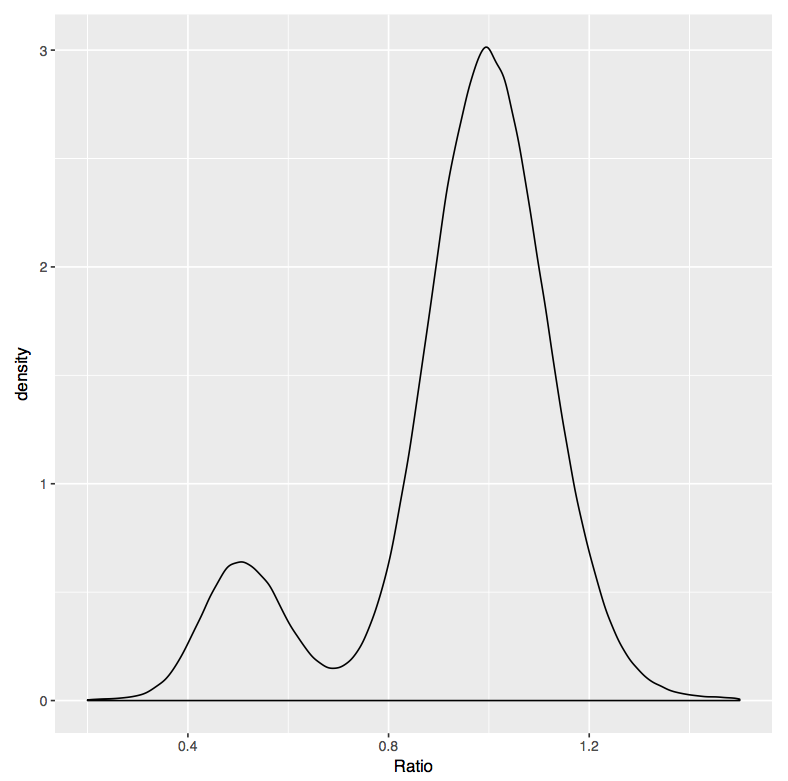
\includegraphics[width=0.5\textwidth]{fg1}
	\caption{Density plot of ratio of read depth in 5kb bins over the average read depth in a diploid organism.}
	\label{fig1} 
\end{figure}

\noindent\textbf{Question 3}: Consider the data shown in Figure \ref{fig1}. The plot shows read depth of bins normalized by the average in a diploid organism. How would you use this data to parametrize the emission probabilities of your HMM? Explain what about Figure 1 is general and what is specific to the data that this plot was derived from. How does this affect the HMM in terms of its application to different data sets? Also, how could this data be utilized to derive the transition probabilities for a CNV detection HMM?\\

\noindent\textbf{Answer}: First, to build a HMM model, we should know each bin's copy number and average depth. We can calculate the emission probabilities by statistic of these informations. For a specified copy number CPX (X = 0,1,2,...). We count how many bins with CPX, assumed N ($N\geq0$). And for each average read depth D (maybe a range), we count the number of bins with the read depth, assumed M. So the emission probability of CPX to read depth D is M/N. 

In Figure 1. The overall appearance of the plot is a Gaussian distribution, which is a general phenomenon in density plot of ratio of read depth plot. In this particular figure, the center ratio (logR) of Gaussian distribution is 1, which reveals the plot derived from a diploid organism. Generally, additional peaks represent alternative copy number states. In this figure, another peak with $logR=0.5$ reveals the particular sample lose some of copies. 

If we build a HMM model base on this sample. The model will have a relatively high transition probability within (CP<2). For other datasets. This will increase the predictions of lose of copy number if apply this to other data sets. 

Computing transition probabilities is similar with computing emission probabilities. Count the changes copy number pairs of adjacent bins. And compute the proportion of the end state from a specified start state.\\

\noindent\textbf{Question 4}: Describe why a HMM, such as discussed in this task is not very useful for non-clonal data (such as shown in Figure 2 below). Could this shortcoming be alleviated by introducing non-integer CN states?

\noindent\textbf{Answer}: As mentioned above, HMM model suppose that copy number state is always integer so it only consider two kinds of clonality 0\% or 100\%. However, for a non-clonal data (such as shown in Figure \ref{fig}). The clonality maybe any value between $0\sim100\%$, and HMM can not return this value.

The shortcoming can not be alleviated by introducing non-integer CN states. First, what number should be used as a state is uncertain. How many states should be used is also uncertain. Besides, introducing non-integer CN states will inevitably increase the number of states and the complexity of model will explode, it will be very time consuming.

\section{Task 2}

The implementation of circular binary segmentation:

First, inputing. Read data from file and build two lists, one is to store the tuple of start and end positions, the other stores the read depths of all bins. 

Second, init the settings. We use numpy to speed up computing. Transfer the list of read depths to numpy array. Then take the median from the first third of the input read depths as `normal' bin m. Transform read depth each bin b into log ratios $log2(b/m)$. Then remove extreme values, specifically, set any log2-ratio that are larger then 2 or smaller than -5 to 0. After this init a segment mark array with 0 for later recursive use. 

Third, a recursive cbs function, this is the most important part of the algorithm. The function have five input parameters: log-ratio array $X$, segment mark array $I$, start position $a$, end position $b$ and z-threshold $t$. For each call of the function. First cut X from a to b, which is the current interval we analyze, name it $X'$. 

Then compute cumulative sum of bins $S_i = X_1+X_2+...+X_i$

After computing cumulative sum. We build a 2d array $Z$ and compute $Z$ by:

\begin{equation*}
Z_{ij}=(\frac{1}{j-i}+\frac{1}{n-j+i})^{-\frac{1}{2}}\times (\frac{S_j-S_i}{j-i}-\frac{S_n-S_j+S_i}{n-j+i})
\end{equation*}

Then find the maximum of $Z$, if the maximum is larger than threshold $t$, its coordinates are new segment points, suppose $x,y$. We mark them in segment mark array I (set corresponding positions to 1) and call three new cbs functions with new interval (a,x),(x,y),(y,b).

Finally, the segment mark array should have marked with 1 in some positions. Find the corresponding interval between two adjacent marks. Compute the average log-ratio and output.

As for the theoretical complexity of the algorithm. For a file with n bins. we compute a $n\times n$ matrix and separate it to 2 segments and compute recursively. So the complexity is:

\begin{equation*}
Complexity = O(n^2 + 2^{1}(\frac{n}{2^{1}})^2 + 2^{2}(\frac{n}{2^{2}})^2+...+2^{t}(\frac{n}{2^{t}})^2)=O(n^2)
\end{equation*}

The complexity mainly scaled with the number of input bins. Of course, the reads depth will also influence it because whether a piece need to be segment decide by them.

\section{Task 3}

\noindent 1. Figure \ref{fig} visualize the reported CNVs. The result of Z equals 10, 1 and 8 shown in Figure \ref{10}, \ref{1}, \ref{8} separately. In these figures, the x axis represent the index of bins, the x coordinate times 5000 and we can get the corresponding positions in reference. The y axis is the log ratio of each bin.

\begin{figure}[h]
	\centering
	\subfigure[Z=10]{
		\label{10}
		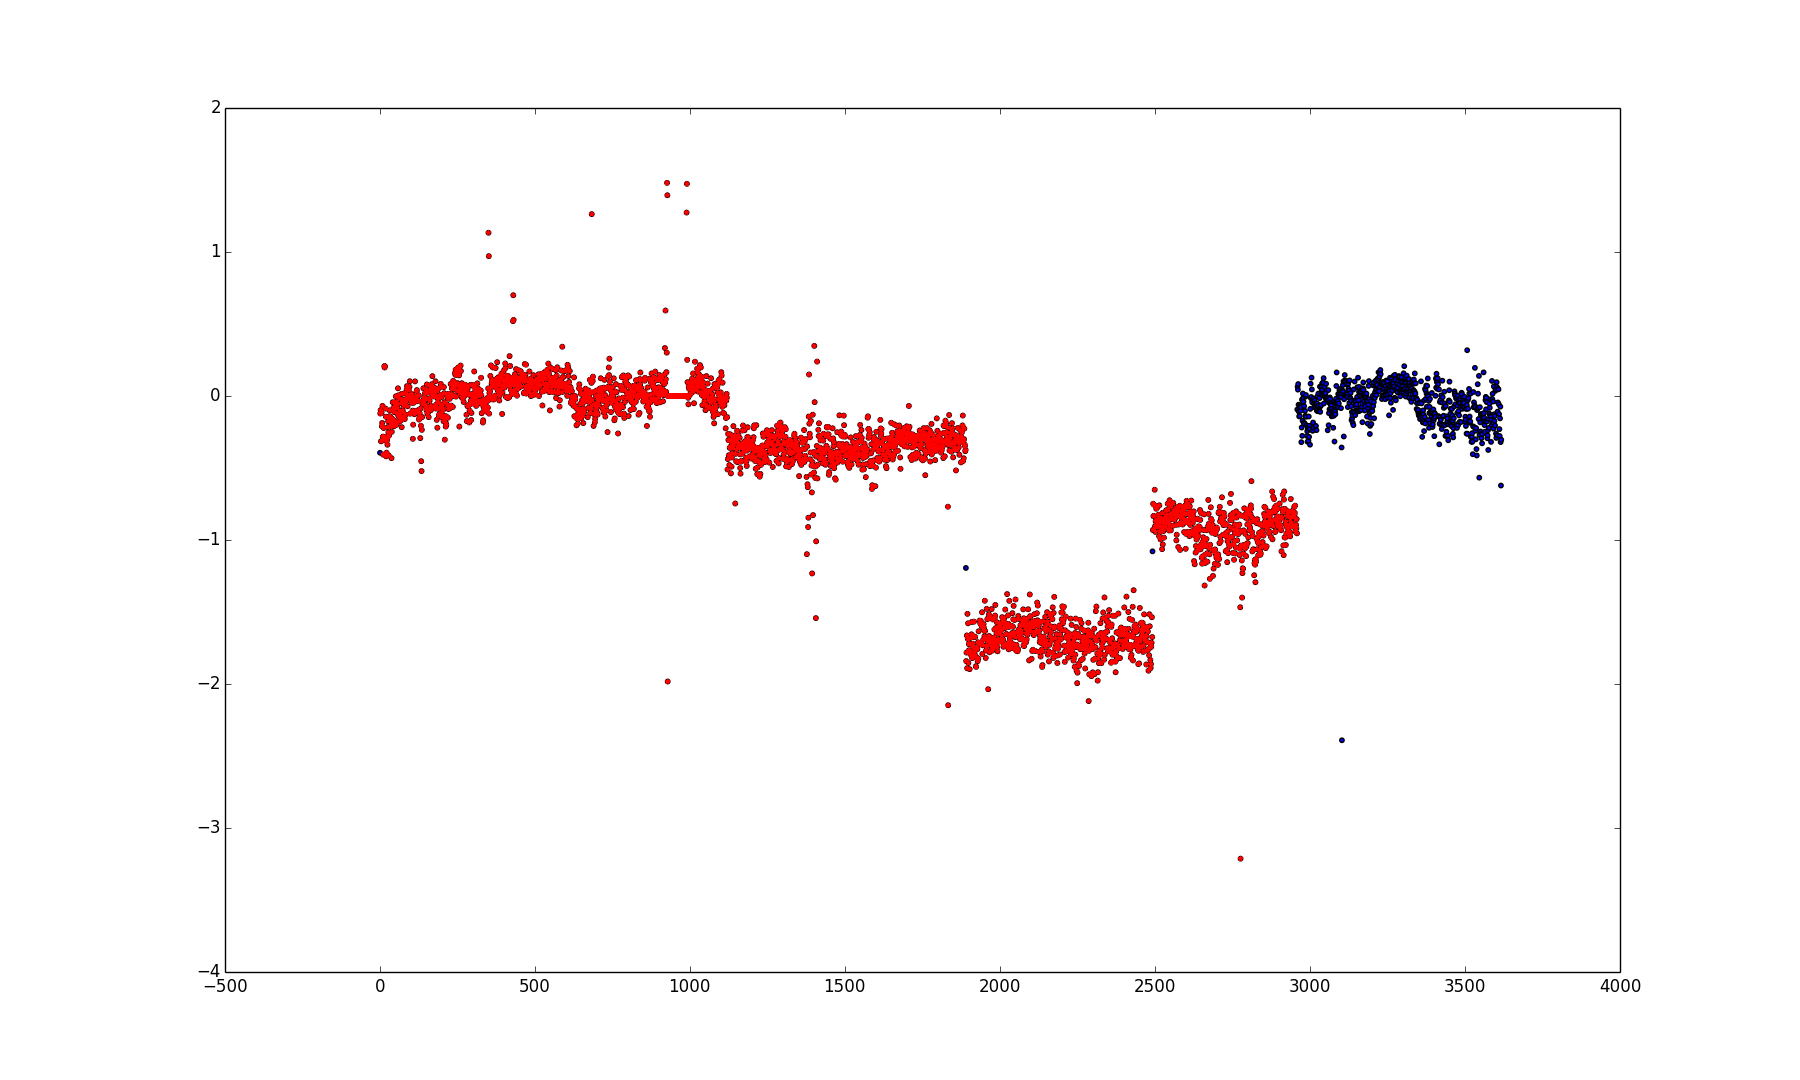
\includegraphics[width=0.8\textwidth]{z10.png}
	}
	\subfigure[Z=1]{
		\label{1}
		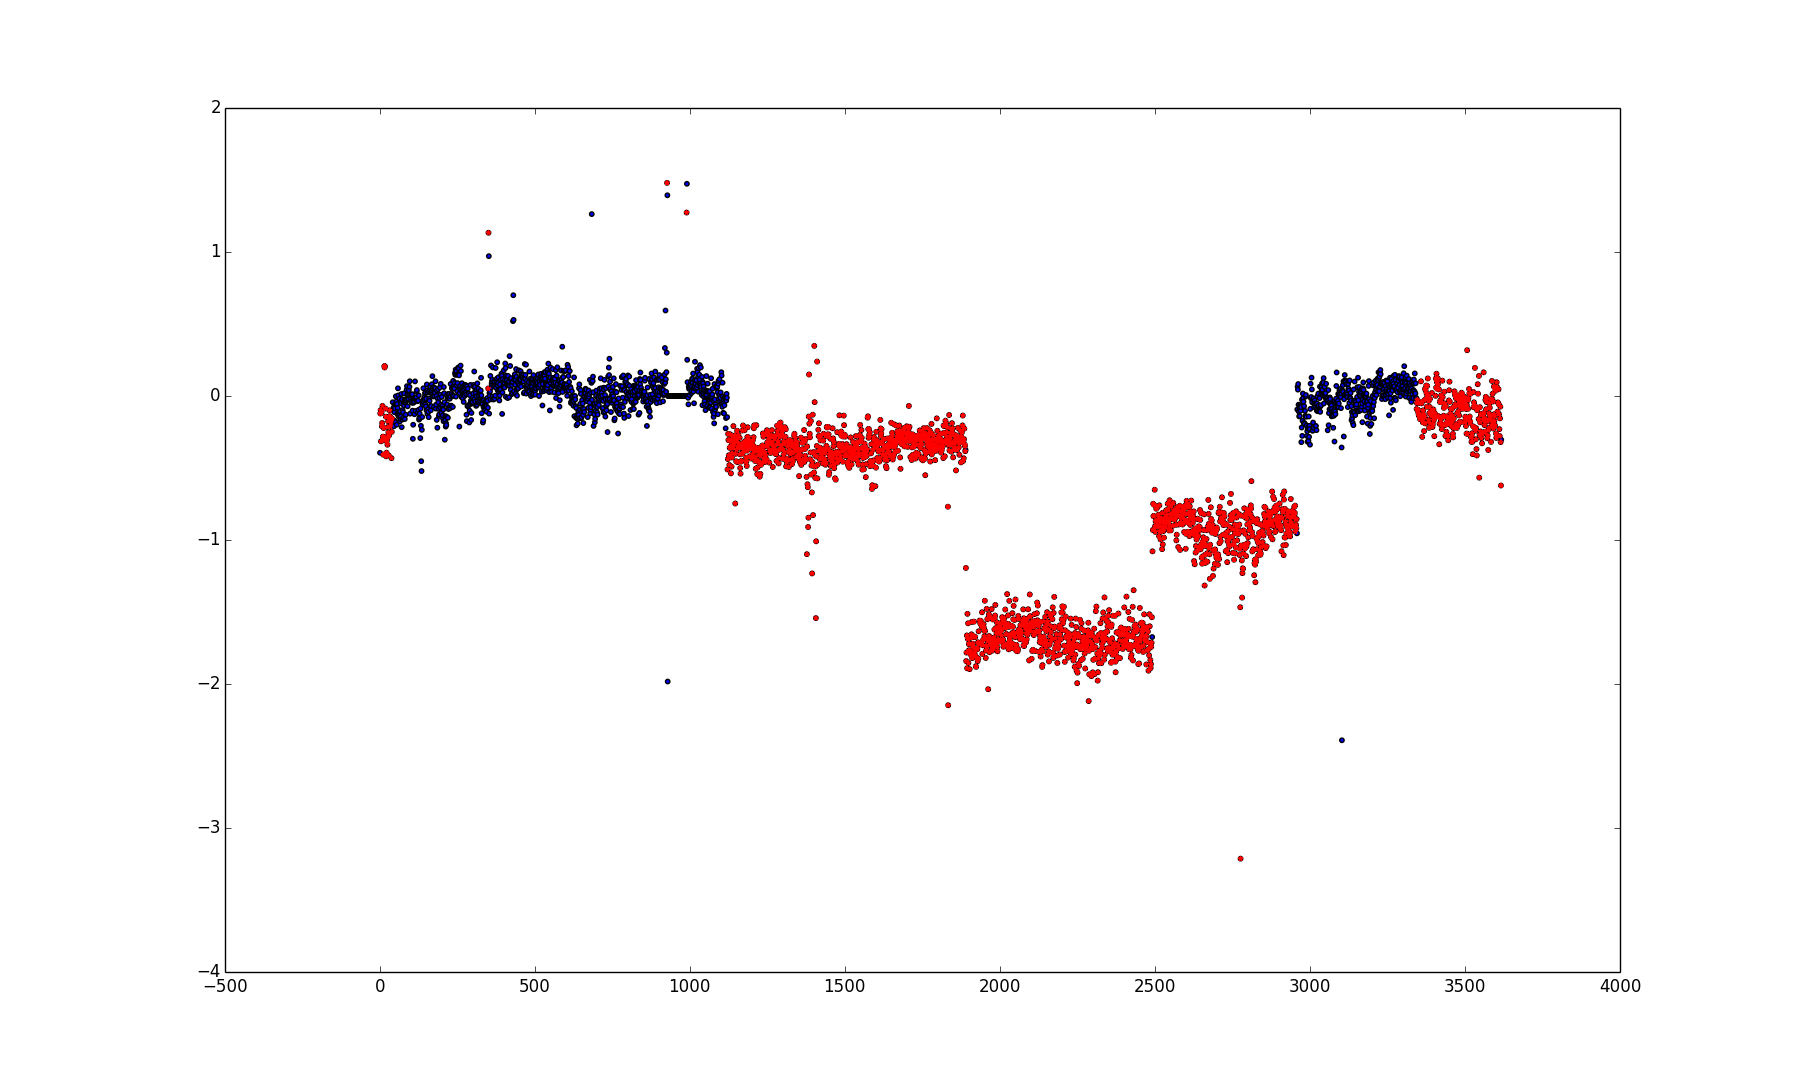
\includegraphics[width=0.45\textwidth]{z1.png}
	}
	\subfigure[Z=8]{
		\label{8}
		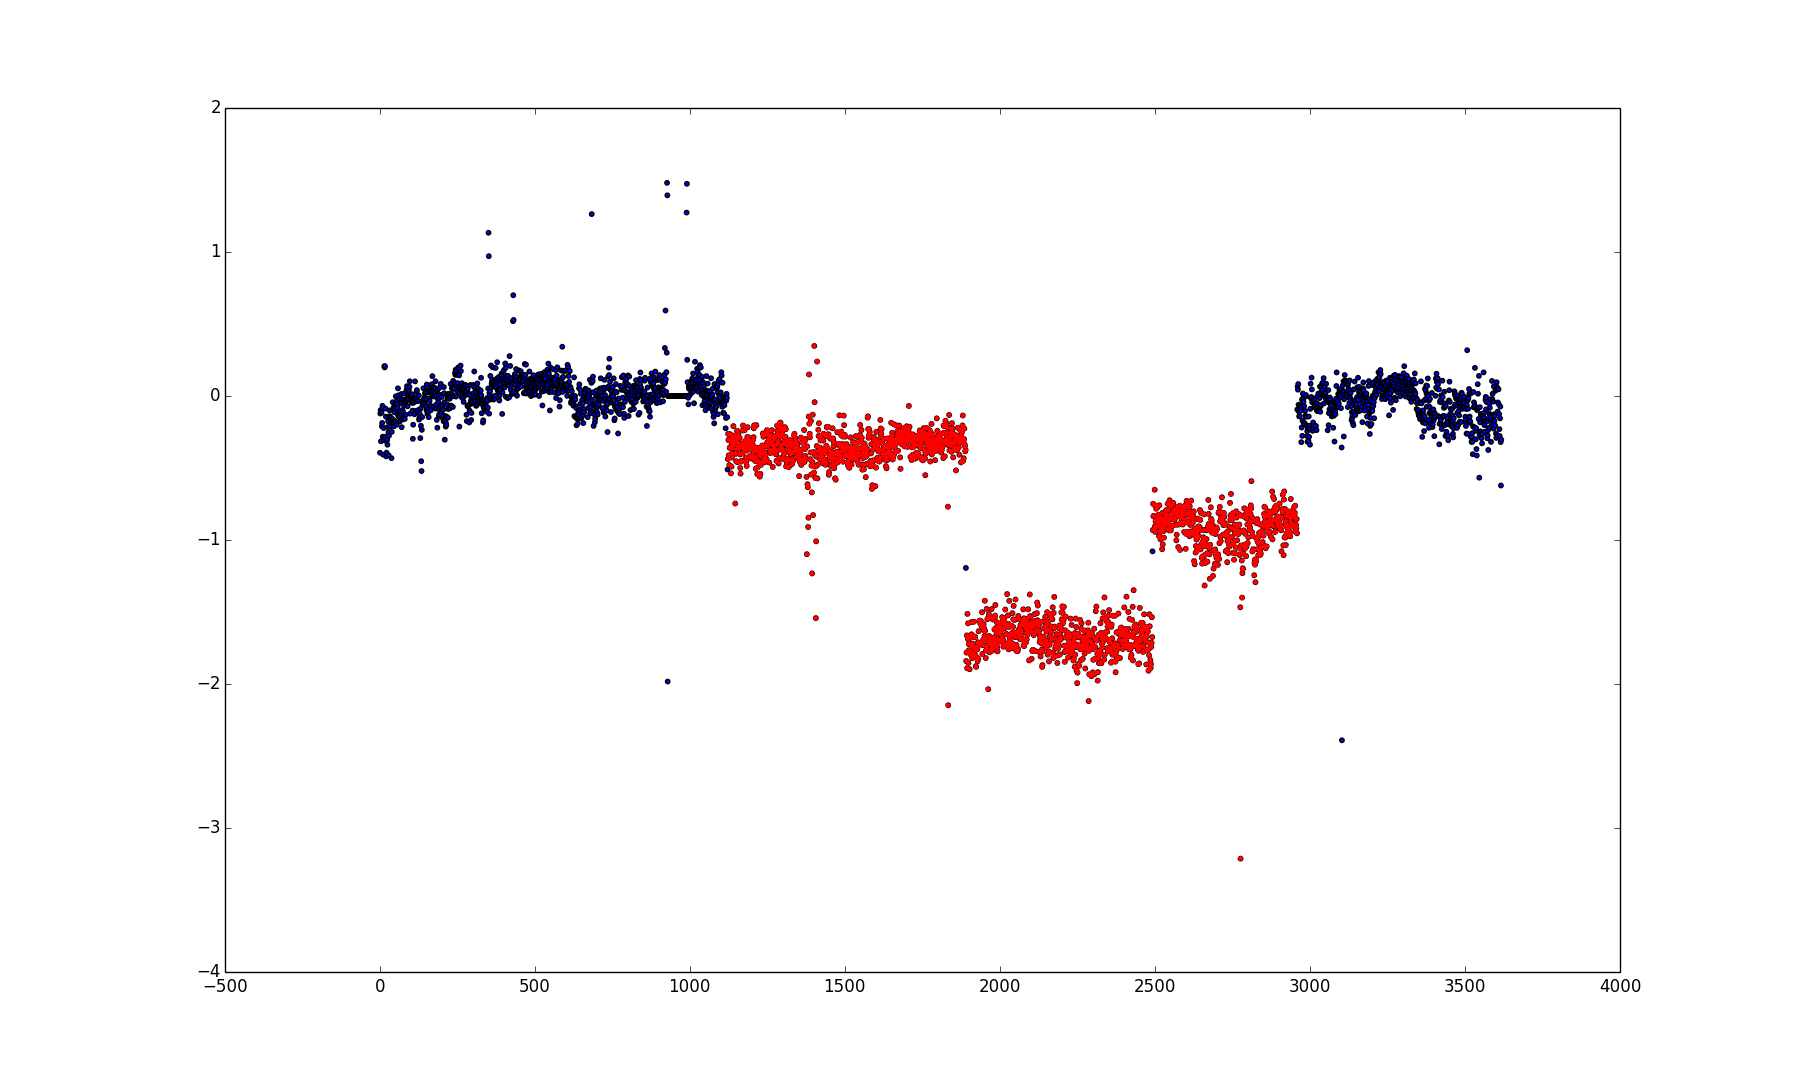
\includegraphics[width=0.45\textwidth]{z8.png}
	}
	\caption{Visualization of CNV. (The red part is reported CNVs)}
	\label{fig} 
\end{figure}

\noindent 2. For $Z=10$, as shown in Figure \ref{10}, we find that no all of the identified CNVs real. The first part, $x$ form 0 to 1800 (0-90Mbp) is not a real CNV, in fact, only $x$ from 1000 to 1800 (50-90Mbp) should be a CNV. In addition, x from 3500 to 3600 (175Mbp-180Mbp) might be false negatives. The average logR is lower than -0.1 and this part does not been detected. To increase sensitivity, we can decrease the Z-threshold, this will lead to more segmentations of the bins meanwhile decreasing the average range of each bins. See Figure \ref{8} and \ref{1}.

\noindent 3. Biology analyze of three large CNVs in the data:

\textbf{a. 50-90Mbp}
\begin{equation*}
logR = -0.3 
\end{equation*}
\begin{equation*}
observed\ copy\ number = 2^{1-0.3}=1.6
\end{equation*}

assume $clonality = c$, with $CN = x$, there is:

\begin{equation*}
xc+2(1-c) = 1.6
\end{equation*}

possible $(x,c)$ pairs:

\begin{equation*}
x = 1, c = 0.4
\end{equation*}
\begin{equation*}
x = 0, c = 0.2
\end{equation*}

\textbf{b. 90-125Mbp}
\begin{equation*}
logR = -1.3 
\end{equation*}
\begin{equation*}
observed\ copy\ number = 2^{1-1.3}=0.8
\end{equation*}

assume $clonality = c$, with $CN = x$, there is:

\begin{equation*}
xc+2(1-c) = 0.8
\end{equation*}

possible $(x,c)$ pairs:

\begin{equation*}
x = 0, c = 0.6
\end{equation*}

\textbf{c. 125-140Mbp}
\begin{equation*}
logR = -0.8
\end{equation*}
\begin{equation*}
observed\ copy\ number = 2^{1-0.3}=1.1
\end{equation*}

assume $clonality = c$, with $CN = x$, there is:

\begin{equation*}
xc+2(1-c) = 1.1
\end{equation*}

possible $(x,c)$ pairs:

\begin{equation*}
x = 1, c = 0.9
\end{equation*}
\begin{equation*}
x = 0, c = 0.45
\end{equation*}

Based on the computed result above, the first and third changes could be both single or double copy losses of the DNA and the second change must be double copy losses of the DNA. Assume three CNVs happens independently on two clones. There are four possible cases for these three CNVs, show in Table \ref{tb:1}

\begin{table}[h]
	\centering
	\begin{tabular}{c|cccccc}
		case\# & $x_1$ & $c_1$ & $x_2$ & $c_2$ & $x_3$ & $c_3$ \\
		\hline
		1 & 0 & 0.2 & 0 & 0.6 & 0 & 0.45 \\
		2 & 0 & 0.2 & 0 & 0.6 & 1 & 0.9 \\
		3 & 1 & 0.4 & 0 & 0.6 & 0 & 0.45 \\
		4 & 1 & 0.4 & 0 & 0.6 & 1 & 0.9 \\
	\end{tabular}
	\label{tb:1}
\end{table}

From the table we can find the first and second changes may happened in different cells because $c_1+c_2$ no larger than 1, while there must be some cells contains the second and third changes because $c_2+c_3$ always larger than 1. For the first and third changes, they may happened in different cell cause there are case that $c_1+c_3$ less than 1. 

As discussed in lecture, BAF could be computed from original BAM file to substantiate our theory. 

Actually, there are too many possible clonal structures and possible distribution in the overall population of cells. Figure \ref{clonal} shows two possible results. From the figure we find subclone must exist in these cells. For example, in Figure \ref{11}, 90 percent cells lose part 3 (the third change) on one chromosome and within these cell, some of them lose part 1 and 2 (first and second changes).
\begin{figure}[h]
	\centering
	\subfigure[Totally 10 cells. 1 (10\%) of total is good. 3 (90\%) of total lose the third changes on one chromsome (within azure square). 6 (60\%) of total lose second changes on both chromosomes (within purple square) and 2 (20\%) of total lose first part on both chromosomes(within yellow square).]{
		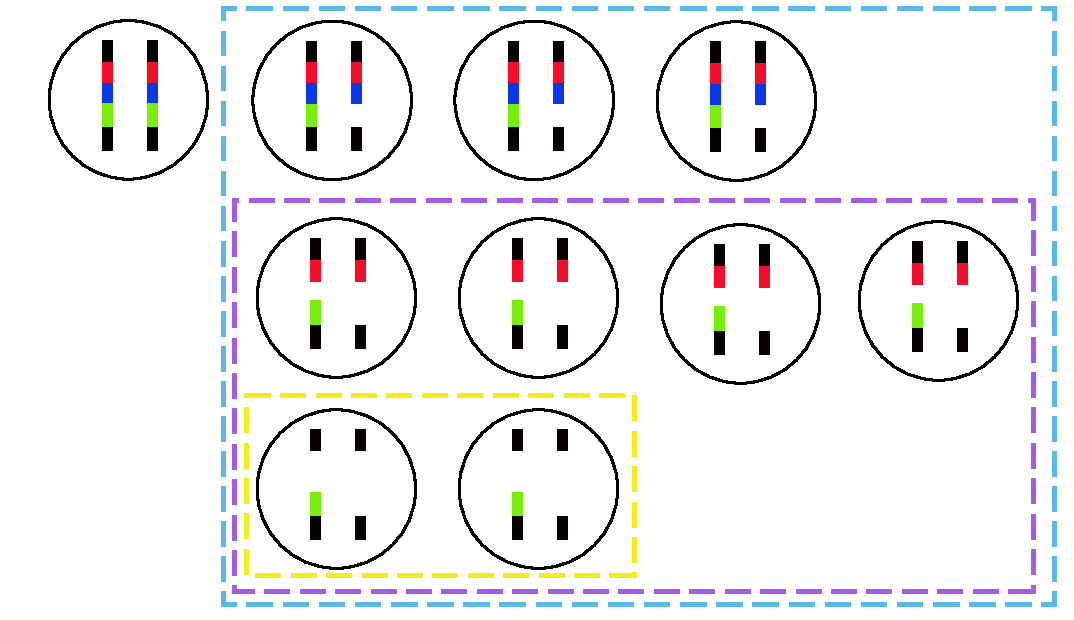
\includegraphics[width=0.75\textwidth]{clonal1.pdf}
		\label{11}
	}
	\subfigure[Totally 10 cells. 1 (10\%) of total is good. 3 (90\%) of total lose the third changes on one chromsome. 6 (60\%) of total lose second changes on both chromosomes and 4 (40\%) of total lose first part on one chromosome.]{
		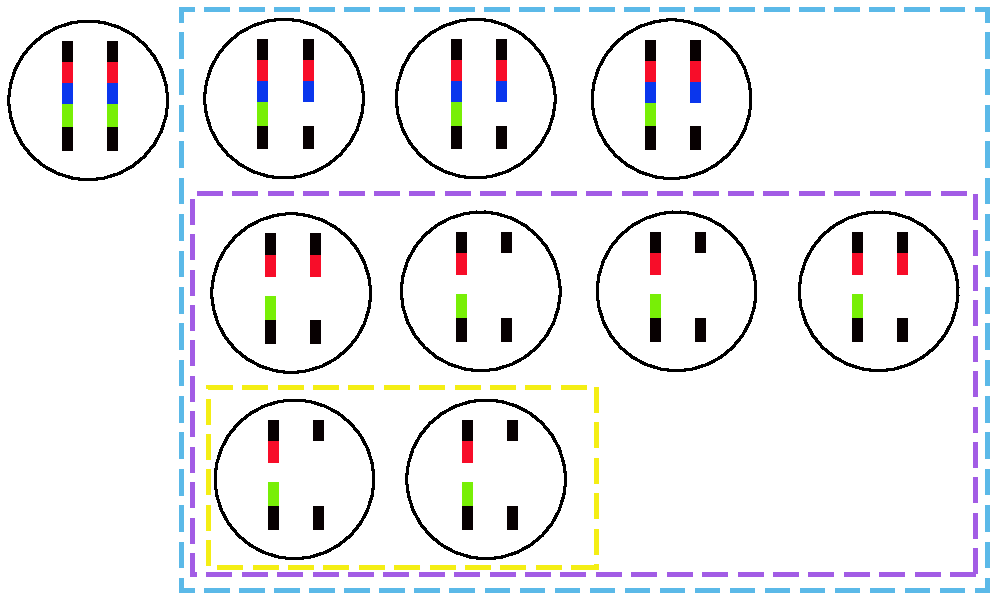
\includegraphics[width=0.75\textwidth]{clonal2.pdf}
	}
	\caption{Possible Clonal structure and its distribution, The red, blue and green part represent first, second and third changes separately. The proportion of each kind of cells represent the proportion in overall population of cells.}
	\label{clonal} 
\end{figure}


%\bibliographystyle{plainnat}
%\bibliography{report}

\end{document}